% ============================================================
%  M²-CL: Multi-Scale & Multi-Layer Contrastive Learning
%  Beamer Presentation  —  Overleaf-compatible
%  Compile with: pdflatex → bibtex → pdflatex × 2
% ============================================================
\documentclass[aspectratio=169,10pt]{beamer}

% ── Theme & Font ────────────────────────────────────────────
\usetheme{Madrid}
\usecolortheme{default}
\usefonttheme{professionalfonts}
\setbeamerfont{title}{size=\Large,series=\bfseries}
\setbeamerfont{frametitle}{size=\normalsize,series=\bfseries}

% ── Custom palette ──────────────────────────────────────────
\definecolor{DarkBlue}{RGB}{26,55,108}
\definecolor{MidBlue}{RGB}{46,117,182}
\definecolor{LightBlue}{RGB}{189,215,238}
\definecolor{AccentOrange}{RGB}{237,125,49}
\definecolor{DarkGray}{RGB}{64,64,64}
\definecolor{LightGray}{RGB}{242,242,242}
\definecolor{GreenOK}{RGB}{112,173,71}

\setbeamercolor{palette primary}{bg=DarkBlue,fg=white}
\setbeamercolor{palette secondary}{bg=MidBlue,fg=white}
\setbeamercolor{palette tertiary}{bg=DarkBlue,fg=white}
\setbeamercolor{palette quaternary}{bg=DarkBlue,fg=white}
\setbeamercolor{structure}{fg=DarkBlue}
\setbeamercolor{frametitle}{bg=DarkBlue,fg=white}
\setbeamercolor{title}{bg=DarkBlue,fg=white}
\setbeamercolor{section in toc}{fg=DarkBlue}
\setbeamercolor{alerted text}{fg=AccentOrange}
\setbeamercolor{block title}{bg=MidBlue,fg=white}
\setbeamercolor{block body}{bg=LightBlue!30,fg=DarkGray}
\setbeamercolor{block title alerted}{bg=AccentOrange,fg=white}
\setbeamercolor{block body alerted}{bg=AccentOrange!15,fg=DarkGray}
\setbeamercolor{block title example}{bg=GreenOK,fg=white}
\setbeamercolor{block body example}{bg=GreenOK!15,fg=DarkGray}

% ── Packages ────────────────────────────────────────────────
\usepackage[utf8]{inputenc}
\usepackage[T1]{fontenc}
\usepackage{lmodern}
\usepackage{amsmath,amssymb,bm}
\usepackage{booktabs}
\usepackage{multirow}
\usepackage{array}
\usepackage{colortbl}
\usepackage{graphicx}
\usepackage{tikz}
\usetikzlibrary{shapes.geometric, arrows.meta, positioning, fit, backgrounds}
\usepackage{pgfplots}
\pgfplotsset{compat=1.18}
\usepackage{xcolor}
\usepackage{hyperref}

% ── Custom commands ─────────────────────────────────────────
\newcommand{\M}{\mathcal{M}}
\newcommand{\Lce}{\mathcal{L}_{\text{CE}}}
\newcommand{\Lcl}{\mathcal{L}^{(l)}}
\newcommand{\ul}{\mathbf{u}^{(l)}}
\newcommand{\highlight}[1]{\textcolor{AccentOrange}{\textbf{#1}}}
\newcommand{\good}[1]{\textcolor{GreenOK}{\textbf{#1}}}
\newcommand{\tablehl}{\rowcolor{LightBlue!60}}

% ── Title info ──────────────────────────────────────────────
\title[M\textsuperscript{2}-CL]{%
  \textbf{M\textsuperscript{2}-CL}\\[4pt]
  Multi-Scale and Multi-Layer Contrastive Learning\\
  for Domain Generalization}
\subtitle{IEEE Transactions on Artificial Intelligence, 2024}
\author[Ballas \& Diou]{%
  Aristotelis Ballas \and Christos Diou\\[6pt]
  {\small \textit{Harokopio University of Athens}}}
\date{arXiv: 2308.14418}
\institute{}

% ── Navigation symbols off ──────────────────────────────────
\setbeamertemplate{navigation symbols}{}
\setbeamertemplate{itemize item}{\color{AccentOrange}$\blacktriangleright$}
\setbeamertemplate{itemize subitem}{\color{MidBlue}$\circ$}

% ── Footer ──────────────────────────────────────────────────
\setbeamertemplate{footline}{%
  \leavevmode%
  \hbox{%
    \begin{beamercolorbox}[wd=.5\paperwidth,ht=2.5ex,dp=1.5ex,left,leftskip=2mm]{palette primary}%
      \usebeamerfont{author in head/foot}%
      \textbf{M\textsuperscript{2}-CL} \;|\; Ballas \& Diou
    \end{beamercolorbox}%
    \begin{beamercolorbox}[wd=.5\paperwidth,ht=2.5ex,dp=1.5ex,right,rightskip=2mm]{palette quaternary}%
      \usebeamerfont{date in head/foot}%
      arXiv:2308.14418 \quad
      \insertframenumber{} / \inserttotalframenumber
    \end{beamercolorbox}}%
}

% ============================================================
\begin{document}
% ============================================================

% ── TITLE ───────────────────────────────────────────────────
\begin{frame}[plain]
  \titlepage
\end{frame}

% ── OUTLINE ─────────────────────────────────────────────────
\begin{frame}{Outline}
  \tableofcontents[hideallsubsections]
\end{frame}

% ============================================================
\section{Problem Statement}
% ============================================================

\begin{frame}{Domain Generalization}
  \begin{columns}[T]
    \column{0.52\textwidth}
      \begin{block}{Challenge}
        \begin{itemize}
          \item Deep CNNs over-fit to \highlight{domain-specific cues}
          \item Distribution shift between train and test
          \item \textbf{No target domain data} during training
        \end{itemize}
      \end{block}
      \vspace{0.4em}
      \begin{alertblock}{Formal Setup}
        Given source domains $\mathcal{D}_1,\ldots,\mathcal{D}_S$, learn a model
        $f_\theta$ that generalizes to \textit{unseen} $\mathcal{D}_T$.
        $$\min_\theta \; \mathbb{E}_{\mathcal{D}_T}\bigl[\mathcal{L}(f_\theta)\bigr]$$
      \end{alertblock}
      \vspace{0.4em}
      \begin{exampleblock}{Real-world impact}
        Medical imaging, autonomous driving, remote sensing
      \end{exampleblock}

    \column{0.44\textwidth}
      \centering
      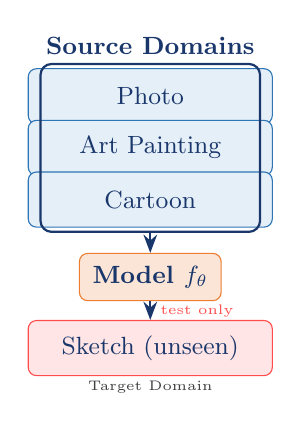
\begin{tikzpicture}[scale=0.82,
        box/.style={draw=MidBlue,fill=LightBlue!40,rounded corners=3pt,
                    minimum width=3.1cm,minimum height=0.7cm,
                    font=\small,text=DarkBlue},
        arrow/.style={-Stealth,thick,DarkBlue}]
        \node[box] (d1) at (0,2.8)  {Photo};
        \node[box] (d2) at (0,2.0)  {Art Painting};
        \node[box] (d3) at (0,1.2)  {Cartoon};
        \draw[thick,DarkBlue,rounded corners] (-1.7,0.7) rectangle (1.7,3.3);
        \node[above,font=\small\bfseries,DarkBlue] at (0,3.3) {Source Domains};
        \node[draw=AccentOrange,fill=AccentOrange!20,rounded corners=3pt,
              minimum width=1.8cm,minimum height=0.6cm,
              font=\small\bfseries,text=DarkBlue] (model) at (0,0) {Model $f_\theta$};
        \draw[arrow] (0,0.7) -- (model);
        \node[draw=red!70,fill=red!10,rounded corners=3pt,
              minimum width=3.1cm,minimum height=0.7cm,
              font=\small,text=DarkBlue] (tgt) at (0,-1.1) {Sketch (unseen)};
        \node[above,font=\small\bfseries,red!70] at (0,-1.55) {};
        \draw[arrow] (model) -- (tgt) node[midway,right,font=\tiny,red!70]{test only};
        \node[font=\tiny,text=DarkGray] at (0,-1.7) {Target Domain};
      \end{tikzpicture}
  \end{columns}
\end{frame}

% ============================================================
\section{Motivation}
% ============================================================

\begin{frame}{Why Multi-Scale \& Multi-Layer?}
  \begin{columns}[T]
    \column{0.48\textwidth}
      \textbf{\color{DarkBlue}Key Insight:} Different network depths encode
      different levels of domain invariance.

      \vspace{0.6em}
      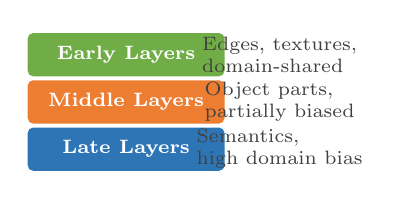
\begin{tikzpicture}[scale=0.75,
        blk/.style={rounded corners=2pt,minimum width=2.5cm,minimum height=0.55cm,
                    font=\scriptsize\bfseries,text=white,align=center}]
        \node[blk,fill=GreenOK] (l1) at (0,2.2)   {Early Layers};
        \node[blk,fill=AccentOrange] (l2) at (0,1.4) {Middle Layers};
        \node[blk,fill=MidBlue]  (l3) at (0,0.6)  {Late Layers};
        \node[font=\scriptsize,text=DarkGray,align=left] at (2.6,2.2)
          {Edges, textures,\\domain-shared};
        \node[font=\scriptsize,text=DarkGray,align=left] at (2.6,1.4)
          {Object parts,\\partially biased};
        \node[font=\scriptsize,text=DarkGray,align=left] at (2.6,0.6)
          {Semantics,\\high domain bias};
      \end{tikzpicture}

      \vspace{0.5em}
      \highlight{Prior work} uses only the \textbf{final layer} representation
      — discarding rich intermediate information.

    \column{0.48\textwidth}
      \begin{block}{M\textsuperscript{2}-CL Hypothesis}
        Jointly leveraging \textbf{all M intermediate layers} and
        \textbf{multiple spatial scales} leads to more robust
        domain-invariant representations.
      \end{block}

      \vspace{0.5em}
      \begin{itemize}
        \item[$\checkmark$] Multi-\textbf{layer}: 13 intermediate conv layers
        \item[$\checkmark$] Multi-\textbf{scale}: pooling at 3 spatial sizes
        \item[$\checkmark$] Contrastive: aligns same-class embeddings
      \end{itemize}
  \end{columns}
\end{frame}

% ============================================================
\section{Method}
% ============================================================

\begin{frame}{M\textsuperscript{2}-CL Architecture Overview}
  \centering
  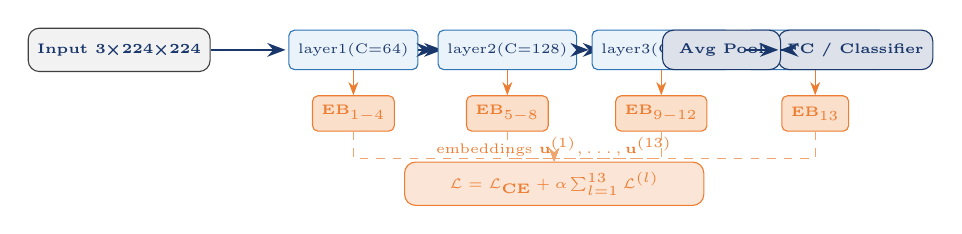
\begin{tikzpicture}[scale=0.85,
    layer/.style={draw=MidBlue,fill=LightBlue!30,rounded corners=2pt,
                  minimum width=1.4cm,minimum height=0.5cm,font=\tiny,text=DarkBlue},
    eb/.style={draw=AccentOrange,fill=AccentOrange!25,rounded corners=2pt,
               minimum width=0.55cm,minimum height=0.45cm,font=\tiny\bfseries,
               text=AccentOrange},
    arrow/.style={-Stealth,thick,DarkBlue,shorten >=1pt}]

    % Input
    \node[draw=DarkGray,fill=LightGray,rounded corners,
          minimum width=1.8cm,minimum height=0.55cm,
          font=\tiny\bfseries,text=DarkBlue] (inp) at (-1.5,0) {Input 3×224×224};

    % Layers
    \foreach \i/\lname/\ch in {1/layer1/64, 2/layer2/128, 3/layer3/256, 4/layer4/512}{
      \node[layer] (L\i) at (\i*2.3-0.3,0) {\lname\\\tiny(C=\ch)};
      \draw[arrow] ([xshift=0.2cm]L\i.east |- 0,0) -- +(0.2,0);
    }
    \draw[arrow] (inp) -- (L1);
    \draw[arrow] (L1) -- (L2);
    \draw[arrow] (L2) -- (L3);
    \draw[arrow] (L3) -- (L4);

    % EB blocks
    \foreach \i/\n in {1/EB$_{1-4}$, 2/EB$_{5-8}$, 3/EB$_{9-12}$, 4/EB$_{13}$}{
      \node[eb] (EB\i) at (\i*2.3-0.3, -0.95) {\n};
      \draw[-Stealth,AccentOrange,thin] (L\i.south) -- (EB\i.north);
    }

    % Classifier
    \node[draw=DarkBlue,fill=DarkBlue!15,rounded corners,
          minimum width=1.5cm,minimum height=0.5cm,
          font=\tiny\bfseries,text=DarkBlue] (cls) at (9.5,0) {FC / Classifier};
    \node[draw=DarkBlue,fill=DarkBlue!15,rounded corners,
          minimum width=1.5cm,minimum height=0.5cm,
          font=\tiny\bfseries,text=DarkBlue] (gap) at (7.5,0) {Avg Pool};
    \draw[arrow] (L4) -- (gap);
    \draw[arrow] (gap) -- (cls);

    % Loss
    \node[draw=AccentOrange,fill=AccentOrange!20,rounded corners,
          minimum width=3.8cm,minimum height=0.55cm,
          font=\tiny\bfseries,text=AccentOrange] (loss) at (5.0,-2.0)
          {$\mathcal{L} = \mathcal{L}_{\text{CE}} + \alpha\sum_{l=1}^{13}\mathcal{L}^{(l)}$};

    \foreach \i in {1,2,3,4}
      \draw[-Stealth,AccentOrange!70,thin,dashed] (EB\i.south) -- +(0,-0.4) -| (loss.north);

    % Embeddings label
    \node[font=\tiny,text=AccentOrange] at (5.0,-1.45) {embeddings $\mathbf{u}^{(1)},\ldots,\mathbf{u}^{(13)}$};
  \end{tikzpicture}

  \vspace{0.4em}
  \small Extraction Blocks (EB) attach to \textbf{13 intermediate layers} and produce
  L2-normalized embeddings used in the contrastive loss.
\end{frame}

\begin{frame}{Extraction Block Design}
  \begin{columns}[T]
    \column{0.44\textwidth}
      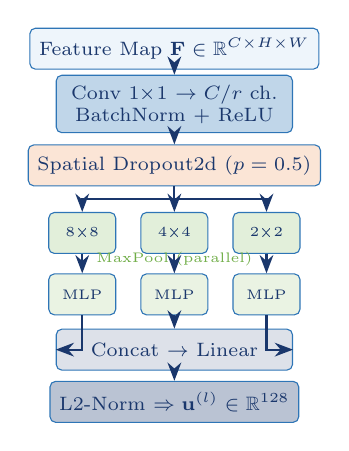
\begin{tikzpicture}[scale=0.78,
        blk/.style={draw=MidBlue,fill=LightBlue!25,rounded corners=2pt,
                    minimum width=3.0cm,minimum height=0.52cm,
                    font=\scriptsize,text=DarkBlue,align=center},
        arrow/.style={-Stealth,thick,DarkBlue}]
        \node[blk] (in)   at (0,5.2) {Feature Map $\mathbf{F}\in\mathbb{R}^{C\times H\times W}$};
        \node[blk,fill=MidBlue!30] (conv) at (0,4.3) {Conv 1×1 $\rightarrow C/r$ ch.\\BatchNorm + ReLU};
        \node[blk,fill=AccentOrange!20] (drop) at (0,3.3) {Spatial Dropout2d $(p=0.5)$};

        % Parallel pools
        \node[blk,fill=GreenOK!20,minimum width=0.85cm] (p1) at (-1.5,2.2) {\tiny 8×8};
        \node[blk,fill=GreenOK!20,minimum width=0.85cm] (p2) at (0,2.2)    {\tiny 4×4};
        \node[blk,fill=GreenOK!20,minimum width=0.85cm] (p3) at (1.5,2.2)  {\tiny 2×2};
        \node[font=\tiny,text=GreenOK] at (0,1.78) {MaxPool (parallel)};

        \node[blk,fill=GreenOK!15,minimum width=0.85cm] (m1) at (-1.5,1.2) {\tiny MLP};
        \node[blk,fill=GreenOK!15,minimum width=0.85cm] (m2) at (0,1.2)    {\tiny MLP};
        \node[blk,fill=GreenOK!15,minimum width=0.85cm] (m3) at (1.5,1.2)  {\tiny MLP};

        \node[blk,fill=DarkBlue!15] (cat) at (0,0.3) {Concat $\rightarrow$ Linear};
        \node[blk,fill=DarkBlue!30] (out) at (0,-0.55) {L2-Norm $\Rightarrow\mathbf{u}^{(l)}\in\mathbb{R}^{128}$};

        \draw[arrow] (in)--(conv); \draw[arrow] (conv)--(drop);
        \draw[arrow] (drop.south) -- +(0,-0.2) -| (p1.north);
        \draw[arrow] (drop.south) -- +(0,-0.2) -| (p2.north);
        \draw[arrow] (drop.south) -- +(0,-0.2) -| (p3.north);
        \foreach \x in {1,2,3} \draw[arrow] (p\x)--(m\x);
        \draw[arrow] (m1.south) |- (cat.west);
        \draw[arrow] (m2)--(cat);
        \draw[arrow] (m3.south) |- (cat.east);
        \draw[arrow] (cat)--(out);
      \end{tikzpicture}

    \column{0.52\textwidth}
      \begin{block}{Components}
        \begin{enumerate}
          \item \textbf{1×1 Conv}: reduce channels by ratio $r{=}4$\\
                $C \to \lfloor C/r \rfloor$
          \item \textbf{Spatial Dropout2d}: drops entire feature maps (not scalars)
          \item \textbf{Parallel Max Pools}:
                \begin{itemize}
                  \item Early layers: $\{8{\times}8,\;4{\times}4,\;2{\times}2\}$
                  \item Late layers: $\{7{\times}7,\;3{\times}3\}$
                \end{itemize}
          \item \textbf{MLP per pipeline} $\to$ fixed-size vector
          \item \textbf{Concat + Linear + L2-norm} $\to \mathbf{u}^{(l)}$
        \end{enumerate}
      \end{block}

      \vspace{0.3em}
      \begin{alertblock}{Why parallel, not cascading?}
        Ablation: parallel $\to 82.83\%$ vs.\ cascading $\to \approx80\%$ (PACS)
      \end{alertblock}
  \end{columns}
\end{frame}

\begin{frame}{Multi-Layer Contrastive Loss}
  \textbf{Per-layer probability measure} for class $c$ at layer $l$:
  \begin{equation*}
    p^{(l)}(c) \;=\;
    \frac{%
      \displaystyle\sum_{\substack{i,j=1\\y_i=y_j=c\\i\neq j}}^{N_c}
        \exp\!\bigl(\mathbf{u}_i^{(l)\top}\mathbf{u}_j^{(l)}/\tau\bigr)
    }{%
      \displaystyle\sum_{\substack{k,m=1\\k\neq m}}^{N_b}
        \exp\!\bigl(\mathbf{u}_k^{(l)\top}\mathbf{u}_m^{(l)}/\tau\bigr)
    }
  \end{equation*}

  \vspace{0.5em}
  \textbf{Layer loss} and \textbf{total loss}:
  \begin{columns}
    \column{0.45\textwidth}
      \begin{alertblock}{}
        \centering
        $\mathcal{L}^{(l)} = -\displaystyle\sum_c \log p^{(l)}(c)$
      \end{alertblock}

    \column{0.50\textwidth}
      \begin{alertblock}{}
        \centering
        $\mathcal{L} = \mathcal{L}_{\text{CE}} + \alpha\displaystyle\sum_{l=1}^{M}\mathcal{L}^{(l)}$
      \end{alertblock}
  \end{columns}

  \vspace{0.6em}
  \begin{columns}
    \column{0.6\textwidth}
      \begin{itemize}
        \item $\mathbf{u}^{(l)}$: L2-normalized embedding from layer $l$
        \item $\tau$: temperature (default $1.0$, stable in $[0.1, 2.0]$)
        \item $\alpha$: loss weight (default $0.01$)
        \item $M = 13$ extraction blocks (ResNet-18)
      \end{itemize}
    \column{0.36\textwidth}
      \begin{exampleblock}{\small Effect of $\alpha$}
        \scriptsize
        $\alpha{=}0.01$: \good{+0.71\% PACS}\\
        $\alpha{=}1.0$: \highlight{$-20\%$ collapse!}
      \end{exampleblock}
  \end{columns}
\end{frame}

% ============================================================
\section{Experimental Setup}
% ============================================================

\begin{frame}{Training Setup \& Hyperparameters}
  \begin{columns}[T]
    \column{0.46\textwidth}
      \begin{block}{Hyperparameters}
        \small
        \begin{tabular}{@{}ll@{}}
          \toprule
          \textbf{Parameter} & \textbf{Value} \\
          \midrule
          Backbone     & ResNet-18 / 50 (ImageNet) \\
          Optimizer    & SGD (momentum 0.9) \\
          LR           & $0.001$ (cosine decay) \\
          Epochs       & $30$ \\
          Batch size   & $128$ \\
          $\alpha$     & $0.01$ \\
          $\tau$       & $1.0$ \\
          $r$          & $4$ \\
          Dropout $p$  & $0.5$ \\
          Embed dim    & $128$ \\
          Hardware     & RTX A5000 \\
          \bottomrule
        \end{tabular}
      \end{block}

    \column{0.50\textwidth}
      \begin{block}{Evaluation Protocol}
        \begin{itemize}
          \item \textbf{Leave-one-domain-out}: each domain serves as the unseen test set
          \item Average top-1 accuracy over \textbf{3 random seeds}
          \item Same train/test splits as \textbf{DomainBed}
          \item Compared against 10 baseline methods
        \end{itemize}
      \end{block}

      \vspace{0.4em}
      \begin{block}{Data Augmentation (DomainBed)}
        \begin{itemize}
          \item Random resized crop $224{\times}224$
          \item Random horizontal flip
          \item Color jitter + random grayscale
          \item ImageNet normalization
        \end{itemize}
      \end{block}
  \end{columns}
\end{frame}

\begin{frame}{Benchmark Datasets}
  \begin{columns}[T]
    \column{0.48\textwidth}
      \begin{block}{PACS}
        \begin{itemize}
          \item 4 domains: Photo, Art, Cartoon, Sketch
          \item $9{,}991$ images, \textbf{7 classes}
        \end{itemize}
      \end{block}
      \vspace{0.3em}
      \begin{block}{VLCS}
        \begin{itemize}
          \item 4 datasets: PASCAL, LabelMe, Caltech-101, SUN09
          \item $10{,}729$ images, \textbf{5 classes}
        \end{itemize}
      \end{block}

    \column{0.48\textwidth}
      \begin{block}{Office-Home}
        \begin{itemize}
          \item 4 domains: Art, Clipart, Product, RealWorld
          \item $15{,}588$ images, \textbf{65 classes}
        \end{itemize}
      \end{block}
      \vspace{0.3em}
      \begin{block}{NICO}
        \begin{itemize}
          \item 19 classes, $25{,}000$ images
          \item Hold out $N \in \{3,5,7\}$ contexts
        \end{itemize}
      \end{block}
  \end{columns}

  \vspace{0.5em}
  \centering
  \small All evaluated with \textbf{leave-one-domain-out} protocol $\cdot$ \textbf{top-1 accuracy}
\end{frame}

% ============================================================
\section{Results}
% ============================================================

\begin{frame}{Results on PACS (ResNet-18)}
  \centering
  \small
  \begin{tabular}{@{}lccccC{1.2cm}@{}}
    \toprule
    \textbf{Method} & \textbf{Art} & \textbf{Cartoon} & \textbf{Photo} & \textbf{Sketch} & \textbf{Avg} \\
    \midrule
    ERM       & 77.37 & 75.51 & 96.11 & 69.27 & 84.51 \\
    RSC       & 75.21 & 74.68 & 95.84 & 75.03 & 80.11 \\
    CORAL     & 76.23 & 77.01 & 93.58 & 70.35 & 84.29 \\
    Mixup     & 78.11 & 73.67 & 94.29 & 74.75 & 84.13 \\
    MMD       & 76.45 & 74.32 & 94.85 & 69.47 & 78.77 \\
    SagNet    & 77.55 & 76.41 & 95.16 & 77.89 & 83.58 \\
    SelfReg   & 77.81 & 76.35 & 95.42 & 74.32 & 80.97 \\
    EQRM      & 79.04 & 75.92 & 94.76 & 73.11 & 80.71 \\
    SAGM      & 79.21 & 77.35 & 94.61 & 79.58 & 82.68 \\
    \midrule
    \tablehl
    \textbf{M\textsuperscript{2}-CL} & \textbf{81.66} & \textbf{78.42} & \textbf{97.00} & 77.07 & \textbf{83.54} \\
    \bottomrule
  \end{tabular}

  \vspace{0.5em}
  \begin{columns}
    \column{0.48\textwidth}
      \begin{alertblock}{\small Key results}
        \small $+0.86\%$ avg over SAGM (2nd best)\\
        Best in Art, Cartoon, Photo
      \end{alertblock}
    \column{0.48\textwidth}
      \begin{exampleblock}{\small Note}
        \small Sketch lags SAGM by $-2.5\%$\\
        Other domains more than compensate
      \end{exampleblock}
  \end{columns}
\end{frame}

\begin{frame}{Results on VLCS (ResNet-18)}
  \centering
  \small
  \begin{tabular}{@{}lccccc@{}}
    \toprule
    \textbf{Method} & \textbf{PASCAL} & \textbf{LabelMe} & \textbf{Caltech-101} & \textbf{SUN09} & \textbf{Avg} \\
    \midrule
    ERM       & 72.11 & 62.14 & 95.47 & 69.11 & 74.71 \\
    CORAL     & 73.42 & 63.88 & 95.32 & 66.70 & 74.83 \\
    Mixup     & 71.88 & 63.45 & 96.21 & 68.43 & 75.00 \\
    SagNet    & 73.87 & 62.69 & 97.33 & 68.04 & 75.48 \\
    SelfReg   & 74.02 & 62.91 & 96.74 & 66.47 & 75.04 \\
    ARM       & 72.54 & 63.11 & 95.87 & 67.39 & 74.73 \\
    EQRM      & 72.76 & 63.20 & 96.43 & 67.88 & 75.07 \\
    SAGM      & 70.97 & 63.56 & 96.81 & 69.33 & 75.17 \\
    \midrule
    \tablehl
    \textbf{M\textsuperscript{2}-CL} & \textbf{73.23} & \textbf{64.12} & \textbf{98.23} & \textbf{75.53} & \textbf{77.78} \\
    \bottomrule
  \end{tabular}

  \vspace{0.4em}
  \begin{alertblock}{\small Key improvement: $+2.61\%$ over second best (SagNet, $75.17\%$)}
    \small Caltech-101: $98.23\%$ ($+1.42\%$) \quad SUN09: $75.53\%$ ($+6.20\%$) — largest gains
  \end{alertblock}
\end{frame}

\begin{frame}{Results on Office-Home \& NICO (ResNet-18)}
  \begin{columns}[T]
    \column{0.54\textwidth}
      \textbf{Office-Home}
      \vspace{0.2em}
      \small
      \begin{tabular}{@{}lccccc@{}}
        \toprule
        \textbf{Method} & \textbf{Art} & \textbf{Clip.} & \textbf{Prod.} & \textbf{Real} & \textbf{Avg} \\
        \midrule
        ERM    & 57.45 & 51.74 & 68.11 & 58.27 & 58.89 \\
        CORAL  & 58.09 & 52.92 & 69.17 & 60.19 & 60.09 \\
        SagNet & 57.12 & 52.28 & 69.34 & 60.05 & 59.70 \\
        SAGM   & 57.92 & 52.65 & 68.95 & 59.12 & 59.66 \\
        \midrule
        \tablehl
        \textbf{M\textsuperscript{2}-CL} & \textbf{58.21} & \textbf{54.02} & \textbf{71.03} & \textbf{69.82} & \textbf{63.27} \\
        \bottomrule
      \end{tabular}

      \vspace{0.3em}
      \begin{alertblock}{\small $+3.61\%$ over CORAL (best baseline)}
      \end{alertblock}

    \column{0.42\textwidth}
      \textbf{NICO}
      \vspace{0.2em}
      \small
      \begin{tabular}{@{}lcccc@{}}
        \toprule
        \textbf{Method} & \textbf{N=3} & \textbf{N=5} & \textbf{N=7} \\
        \midrule
        ERM     & 66.77 & 64.11 & 59.10 \\
        CORAL   & 66.45 & 64.39 & 59.43 \\
        SagNet  & 66.12 & 64.77 & 60.22 \\
        SAGM    & 66.77 & 65.00 & 59.10 \\
        \midrule
        \tablehl
        \textbf{M\textsuperscript{2}-CL} & \textbf{68.43} & \textbf{65.87} & \textbf{62.19} \\
        \bottomrule
      \end{tabular}

      \vspace{0.3em}
      \begin{exampleblock}{\small N=7: $+3.09\%$ most challenging}
      \end{exampleblock}
  \end{columns}
\end{frame}

% ============================================================
\section{Ablation Study}
% ============================================================

\begin{frame}{Ablation: Architecture Components}
  \begin{columns}[T]
    \column{0.54\textwidth}
      \small
      \begin{tabular}{@{}lcc@{}}
        \toprule
        \textbf{Configuration} & \textbf{PACS} & \textbf{VLCS} \\
        \midrule
        Full M\textsuperscript{2}-CL (+ loss)  & \good{83.54} & \good{77.78} \\
        M\textsuperscript{2} only (no CL loss) & 82.83        & 76.11 \\
        \midrule
        Cascading pipelines        & 80.12 & 73.45 \\
        \highlight{No spatial dropout}      & 80.89 & 73.18 \\
        \midrule
        $r=2$ (more channels)      & 81.73 & 75.34 \\
        $r=4$ \textit{(default)}   & \good{82.83} & \good{76.11} \\
        $r=6$ (fewer channels)     & 81.44 & 74.98 \\
        \bottomrule
      \end{tabular}

    \column{0.42\textwidth}
      \begin{block}{Key takeaways}
        \begin{itemize}
          \item \textbf{Parallel} beats cascading by $\approx 2.7\%$
          \item \textbf{Spatial dropout} is critical: $+2\%$ on VLCS
          \item \textbf{CL loss} adds $+0.71\%$ (PACS) and $+1.67\%$ (VLCS)
          \item $r=4$ is the sweet spot
        \end{itemize}
      \end{block}
      \vspace{0.3em}
      \begin{alertblock}{\small Insight}
        Spatial Dropout forces the model to rely on
        \textit{distributed} features, not single channels
      \end{alertblock}
  \end{columns}
\end{frame}

\begin{frame}{Ablation: Hyperparameter Sensitivity}
  \begin{columns}[T]
    \column{0.50\textwidth}
      \textbf{Temperature $\tau$}
      \vspace{0.2em}
      \small
      \begin{tabular}{@{}lcc@{}}
        \toprule
        $\tau$ & \textbf{PACS} & \textbf{VLCS} \\
        \midrule
        0.01   & 80.12 & 73.98 \\
        0.1    & 81.67 & 76.02 \\
        0.5    & 82.93 & 77.11 \\
        \good{1.0} \textit{(default)} & \good{83.54} & \good{77.78} \\
        2.0    & 83.31 & 77.61 \\
        10     & 82.01 & 75.44 \\
        100    & 78.34 & 73.21 \\
        \bottomrule
      \end{tabular}

      \vspace{0.3em}
      \begin{exampleblock}{\small $\tau \in [0.5,2.0]$: stable ($\pm 0.23\%$)}
      \end{exampleblock}

    \column{0.46\textwidth}
      \textbf{Loss weight $\alpha$}
      \vspace{0.2em}
      \small
      \begin{tabular}{@{}lcc@{}}
        \toprule
        $\alpha$ & \textbf{PACS} & \textbf{VLCS} \\
        \midrule
        $10^{-5}$ & 82.80 & 76.08 \\
        $10^{-3}$ & 82.99 & 76.45 \\
        \good{$0.01$} \textit{(default)} & \good{83.54} & \good{77.78} \\
        $0.1$     & 82.23 & 76.91 \\
        \highlight{$1.0$} & \highlight{63.54} & \highlight{57.22} \\
        \bottomrule
      \end{tabular}

      \vspace{0.3em}
      \begin{alertblock}{\small $\alpha=1.0$ destroys training!\\CE and CL severely imbalanced.}
      \end{alertblock}
  \end{columns}
\end{frame}

% ============================================================
\section{Conclusion}
% ============================================================

\begin{frame}{Conclusion}
  \begin{columns}[T]
    \column{0.54\textwidth}
      \begin{block}{Contributions}
        \begin{itemize}
          \item[\good{$\checkmark$}] \textbf{Extraction blocks} on 13 ResNet layers with parallel concentration pipelines
          \item[\good{$\checkmark$}] \textbf{Spatial Dropout} forces distributed representations
          \item[\good{$\checkmark$}] \textbf{Multi-layer contrastive loss} aligns same-class embeddings at every scale
          \item[\good{$\checkmark$}] SotA on all 4 benchmarks: \good{PACS, VLCS, Office-Home, NICO}
        \end{itemize}
      \end{block}

      \vspace{0.3em}
      \begin{exampleblock}{Summary of gains (ResNet-18)}
        \small
        \begin{tabular}{@{}lcc@{}}
          \toprule
          Dataset & Ours & $\Delta$ \\
          \midrule
          PACS        & 83.54\% & $+0.86\%$ \\
          VLCS        & 77.78\% & $+2.61\%$ \\
          Office-Home & 63.27\% & $+3.61\%$ \\
          NICO (N=7)  & 62.19\% & $+3.09\%$ \\
          \bottomrule
        \end{tabular}
      \end{exampleblock}

    \column{0.42\textwidth}
      \begin{alertblock}{Future Work}
        \begin{itemize}
          \item Extend to \textbf{ViT / Transformer} backbones
          \item Semi-supervised DG
          \item Video domain generalization
          \item Few-shot adaptation
        \end{itemize}
      \end{alertblock}

      \vspace{0.6em}
      \begin{block}{Code \& Paper}
        \small
        arXiv: \texttt{2308.14418}\\[4pt]
        IEEE Trans.\ AI, 2024
      \end{block}
  \end{columns}
\end{frame}

% ── REFERENCES ──────────────────────────────────────────────
\begin{frame}[allowframebreaks]{References}
  \small
  \begin{thebibliography}{9}
    \bibitem{m2cl}
      A.~Ballas and C.~Diou,
      ``M\textsuperscript{2}-CL: Multi-Scale and Multi-Layer Contrastive Learning for Domain Generalization,''
      \emph{IEEE Trans.\ Artif.\ Intell.}, 2024. arXiv:2308.14418.

    \bibitem{domainbed}
      I.~Gulrajani and D.~Lopez-Paz,
      ``In Search of Lost Domain Generalization,''
      \emph{ICLR}, 2021.

    \bibitem{resnet}
      K.~He et al.,
      ``Deep Residual Learning for Image Recognition,''
      \emph{CVPR}, 2016.

    \bibitem{simclr}
      T.~Chen et al.,
      ``A Simple Framework for Contrastive Learning of Visual Representations,''
      \emph{ICML}, 2020.

    \bibitem{pacs}
      D.~Li et al.,
      ``Deeper, Broader and Artier Domain Generalization,''
      \emph{ICCV}, 2017.

    \bibitem{supcon}
      P.~Khosla et al.,
      ``Supervised Contrastive Learning,''
      \emph{NeurIPS}, 2020.

    \bibitem{sagm}
      Q.~Wang et al.,
      ``SAGM: Sharpness-Aware Gradient Matching for Domain Generalization,''
      \emph{CVPR}, 2023.

    \bibitem{coral}
      B.~Sun and K.~Saenko,
      ``Deep CORAL: Correlation Alignment for Deep Domain Adaptation,''
      \emph{ECCV Workshops}, 2016.
  \end{thebibliography}
\end{frame}

\end{document}
